\section{Work method}
The strategy is selected according to the principles presented in the Object-Oriented Analysis \& Design (OOA\&D) method.
This method is used to analyze and more importantly understand a problem in a way that enables determining requirements and developing a system without significant uncertainties.

To avoid those uncertainties the method emphasises post-poning non-critical decisions as a way to maintain the freedom to make these choices at a later time, where more information is available and the risk of uncertainties therefore is lower.
Same reasoning applies to the principle of beginning the work in the area that poses the greatest challenge to the development. 
%Anja: Præsenter OOA&D metoden før du nævner den. 
%Astrid: Sufficient? Vil heller ikke bruge for lang tid på at præsentere noget der først skal bruges meget senere.

% I don't understand the next sentence here.
%better???
% Taniya: does the set of questions have a name?
%dont think so
A set of questions supposed to serve as a starting point for determining which area that is, is provided in the book [p.X, Y].
The questions are answered so that a yes equals to zero points, a maybe to one point and a no to two points.
If the answer is unknown it is counted as a no. The more points an area has the more critical the corresponding area is. The list of these questions and answers can be found in appendix XX.
% Henrik: Synes ikke der burde var BLANK linie her, da de to afsnit hænger sammen
Based on this activity it was concluded that AAA is the most difficult area, with BBB as number two and CCC last.

% Maybe a sort of chapter division here?
% Anja: Generelt skal den ovenstående tekst stå et andet sted. Informationen virker lidt malplaceret.
Selection of a general work structure depends on the degrees of structure and complexity in the project. The waterfall model, where one part of the project is completely finished before the next one is begun is great for projects with low uncertainty and high complexity. However an iterative approach where every part of the project is revisited  multiple times is better for projects with high uncertainty and low complexity. [how does one refer to things the teacher has said but which are not in his own damned book?] % I think you have to find a book that says it

The user is someone who works with handbooks in a professional setting and therefore either has or quickly gains a lot of experience. The task is very structured and one of the main purposes of the system is to make sure that the books remain structured in the face of human errors. The developers on the project however are students with limited experience, which is what provides the most uncertainty to this project. %Anja: Jeg synes ikke, at vi skal skrive, at grunden til at, der er "uncertainty" i projektet pga., at vi er studerende. Det er mere fordi at selve designprocessen i sig selv er usikker/omskiftelig. Hele grundlaget for at have en 'design'-proces til at starte med er, at vi ikke ved hvordan slutproduktet skal se ud på forhånd; derfor er projektet "uncertain".
% Henrik: Hvad er det "the developers" har limited experience med?

The size of the project can be adjusted until it fits the length of the project period and the amount of users is relatively low: There is only one main user and a few who are not as involved. The amount of the new information is very high at the beginning of the project but once understood the complexity is insignificant.

As both the uncertainty and complexity of the project are relatively low, both methods can be used. As there is a high complexity in the very beginning of the project the waterfall method will be used here with an iterative process in the remaining parts of the project to make sure the terms were not misunderstood and to deliver the best possible system to the users. %Nævn gerne noget med designprocessen her.
%Anja: Ellers er teksten fin (y)
% Henrik: Måske flyt dette afsnit op sammen med det tidligere afsnit, hvor der snakkes om "unvertainty and complexity"?

\todo[inline]{Vi skal måske have snakket om placeringen af denne tekst igen. Jeg synes, at den kommer lidt malplaceret ift. indledning. Jeg synes, at det giver mere mening efter problemanalysen.}


\subsection{Iterative design process}
The benefit of working with iteratively is to continually talk with the users and discuss their needs and wants, determine or redetermine requirements. and design a system which gets refined along the way. This ongoing communication with the users and their needs is likewise the center of user-centered approach where there’s a focus on the user’s tasks, empirical measurement and iterative design. (Sharp, Rogers \& Preece)

There are four basic activities when working interaction design which are; \textit{establishing requirements, designing alternatives, prototyping,} and \textit{evaluating}. To be able to design a system with the user’s needs and wants in mind it is imperative to know the target users and which activities the system needs to support. This is done through establishing requirements where information of the target users is gathered through data gathering and analysis. When the requirements are settled it is possible to design alternatives where ideas a suggested that meet these requirements. Here a conceptual design is formed which describes an abstract outline of how the users can interact with it. Concrete designs infers to the details of the design; which could include colors, sounds, images etc. (Sharp, Rogers \& Preece)

When the design alternative phase is complete a prototype can be developed. The purpose of the prototype is to evaluate with the users whether the criteria has been met and give them an idea of how the system could potentially turn out. The prototype doesn’t necessarily have to consist of a working piece of software; the prototype could also be paper-based in the early stages of the design process. When the prototype is complete then it can be measured an evaluated. The evaluation phase determines whether or not the design is usable and/or acceptable. (Sharp, Rogers \& Preece)

\subsubsection{A simple lifecycle model}
All of the before-mentioned activities are related in an iterative design process. This is shown visually in figure xx. The lifecycle model is a simplified version of reality and isn’t meant to be prescriptive, and depending on the project it isn’t always possible to go through all of the phases described. Though the model is developed through Sharp, Rogers and Preece’s research of how software engineering is practiced in the field. (Sharp, Rogers \& Preece)

\begin{figure}[h]
	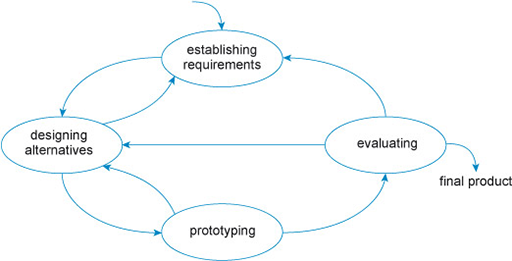
\includegraphics[width=1\textwidth]{billeder/lifecycle.png}
	\caption{Lifecycle model}
\end{figure}

According to Sharp, Rogers and Preece “Most projects start with establishing requirements” (p. 333). It is from this first activity that it’s possible to go into the ‘designing alternatives’ activity from where a prototype. in the ‘prototyping’ activity, can be developed which in turn can be evaluated by the users in the ‘evaluating’ activity. From this evaluation the designers can specify new or redefined requirements, or they can go directly to redesign or deem the project done.

\subsubsection{Using of the lifecycle model in the project}
Throughout the project it is intended to design a system iteratively with a specific user’s needs and wants integrated into the designs and tests. This is the basis of choosing to work with the lifecycle model as a model to reflect over which activity is being used throughout the stages of the project. The lifecycle model is likewise a good indicator of when an iteration is done and when a new one has been commenced. 

As mentioned by Sharp, Rogers and Preece most projects starts with establishing requirements, which will be reflected in this project with an initial interview where the first requirements will be determined. This is intended to result in a following design process and prototype which can be evaluated with the user in a second interview.

% Anja: Jeg kunne ikke lige ellers finde ud af, hvor teksten skulle stå, så jeg satte den ind her